\documentclass[a4paper]{article}

\usepackage[utf8]{inputenc}
\usepackage[portuguese]{babel}
\usepackage{a4wide}
\usepackage[pdftex]{hyperref}
\usepackage{graphicx}
\usepackage{wrapfig}
\usepackage{amsmath}
\usepackage{verbatim}
\usepackage{caption}
\usepackage{subcaption}
\usepackage{float}
\usepackage{blochsphere}
\usepackage{amsfonts}
\usepackage{listings} 
\usepackage{color}

\definecolor{codegreen}{rgb}{0,0.6,0}
\definecolor{codegray}{rgb}{0.5,0.5,0.5}
\definecolor{codepurple}{rgb}{0.58,0,0.82}
\definecolor{backcolour}{rgb}{0.95,0.95,0.92}
\definecolor{white}{rgb}{1,1,1}

\lstdefinestyle{mystyle}{
    backgroundcolor=\color{backcolour},   
    commentstyle=\color{codegreen},
    keywordstyle=\color{magenta},
    numberstyle=\tiny\color{codegray},
    stringstyle=\color{codepurple},
    basicstyle=\footnotesize,
    breakatwhitespace=false,         
    breaklines=true,                 
    captionpos=b,                    
    keepspaces=true,                 
    numbers=left,                    
    numbersep=5pt,                  
    showspaces=false,                
    showstringspaces=false,
    showtabs=false,                  
    tabsize=2
}
 
\lstset{style=mystyle}


\begin{document}

\begin{titlepage}
\begin{center}



\includegraphics[width=0.4\textwidth]{logo.jpg}\\[0.5cm]

\vspace{10mm}

{\huge Universidade do Minho - Escola de Engenharia}\\[0.5cm]

{\large Relatório do trabalho prático de Computação Gráfica}\\[0.5cm]

\vspace{10mm} 

% Title
\rule{\linewidth}{0.5mm} \\[0.4cm]
{ \huge \bfseries Fase 4 – Normais e Coordenadas de texturas \\[0.4cm] }
\rule{\linewidth}{0.5mm} \\[1.5cm]

% Author and supervisor
\noindent
\begin{minipage}{0.4\textwidth}
  \begin{flushleft} \large
    \emph{Autores :}\\
    Daniel Maia \textsc{(A77531)}\\
    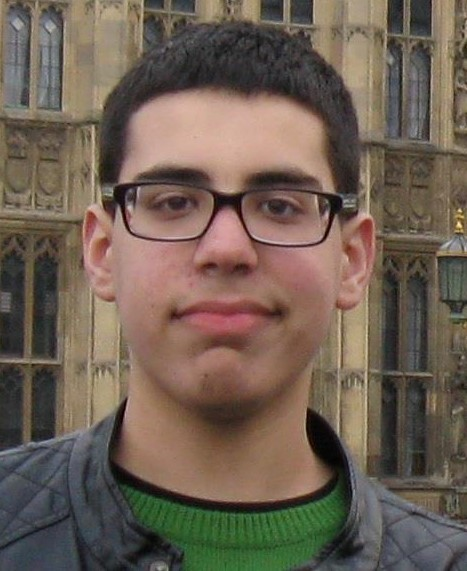
\includegraphics[width=1.5cm]{daniel.jpg}\break
    Diogo Costa\textsc{(A78034)}\\
    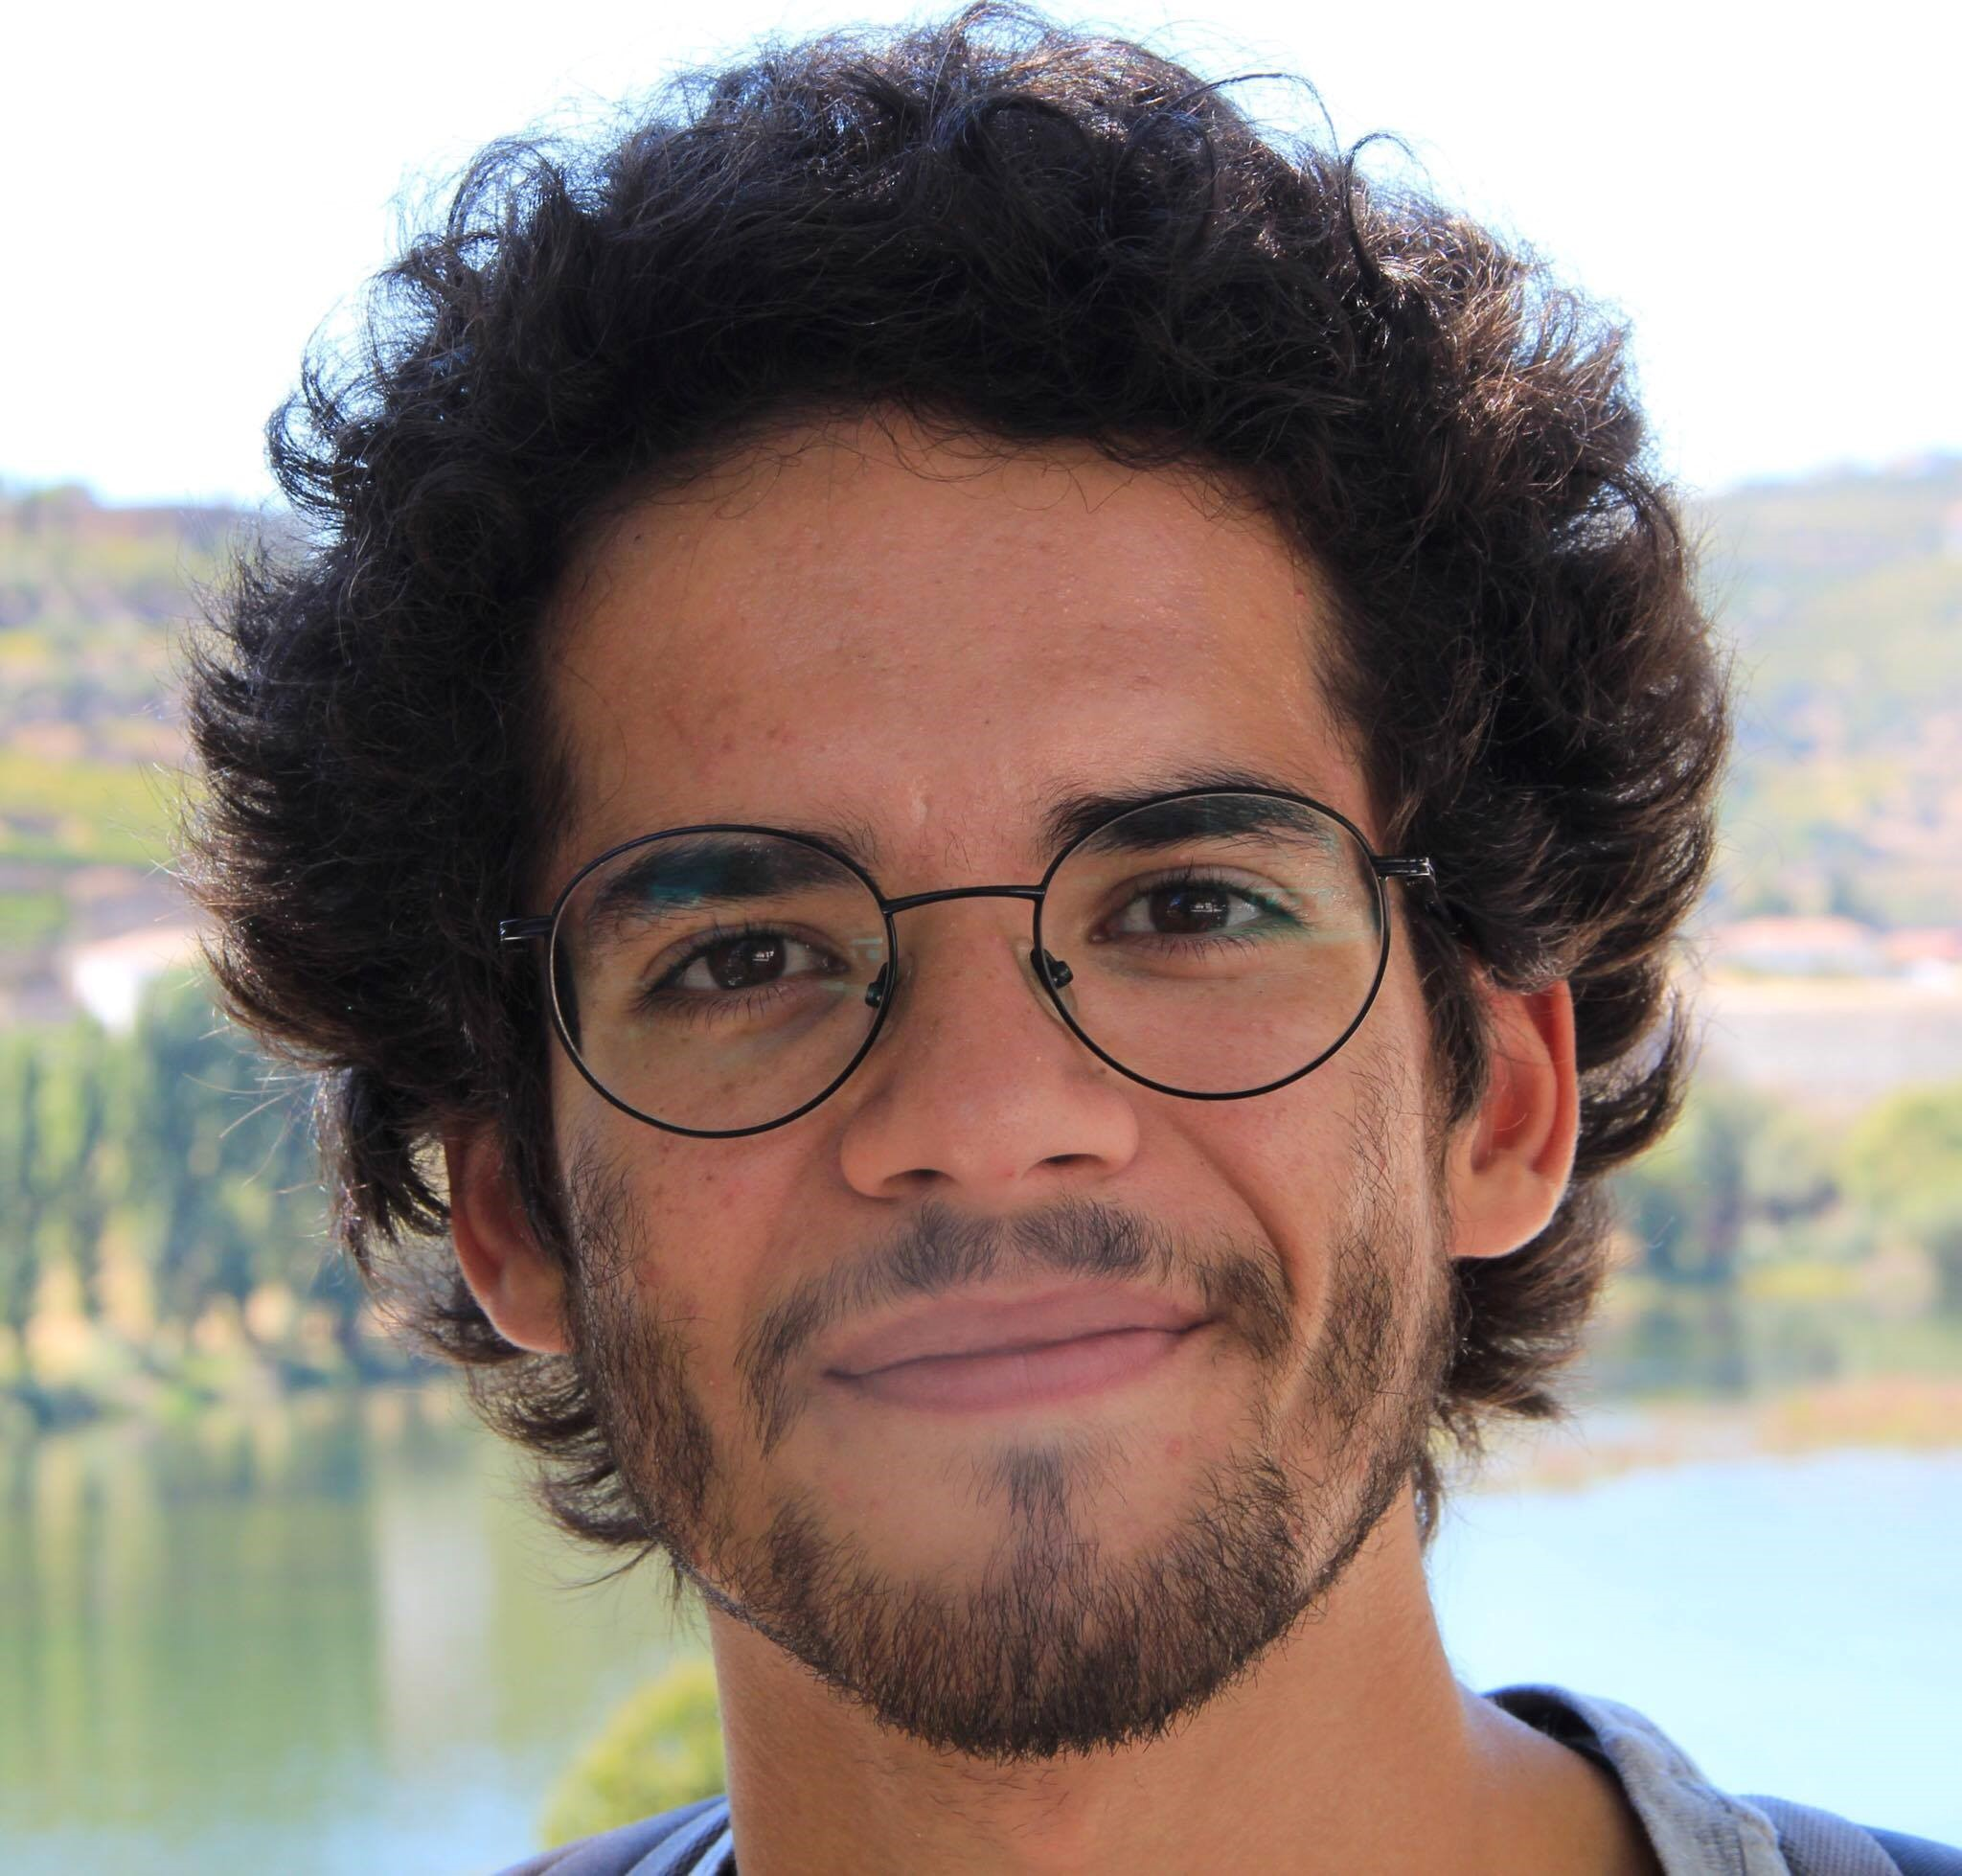
\includegraphics[width=1.5cm]{afonso.jpg}\break
    Marco Silva\textsc{(A79607)}\\
    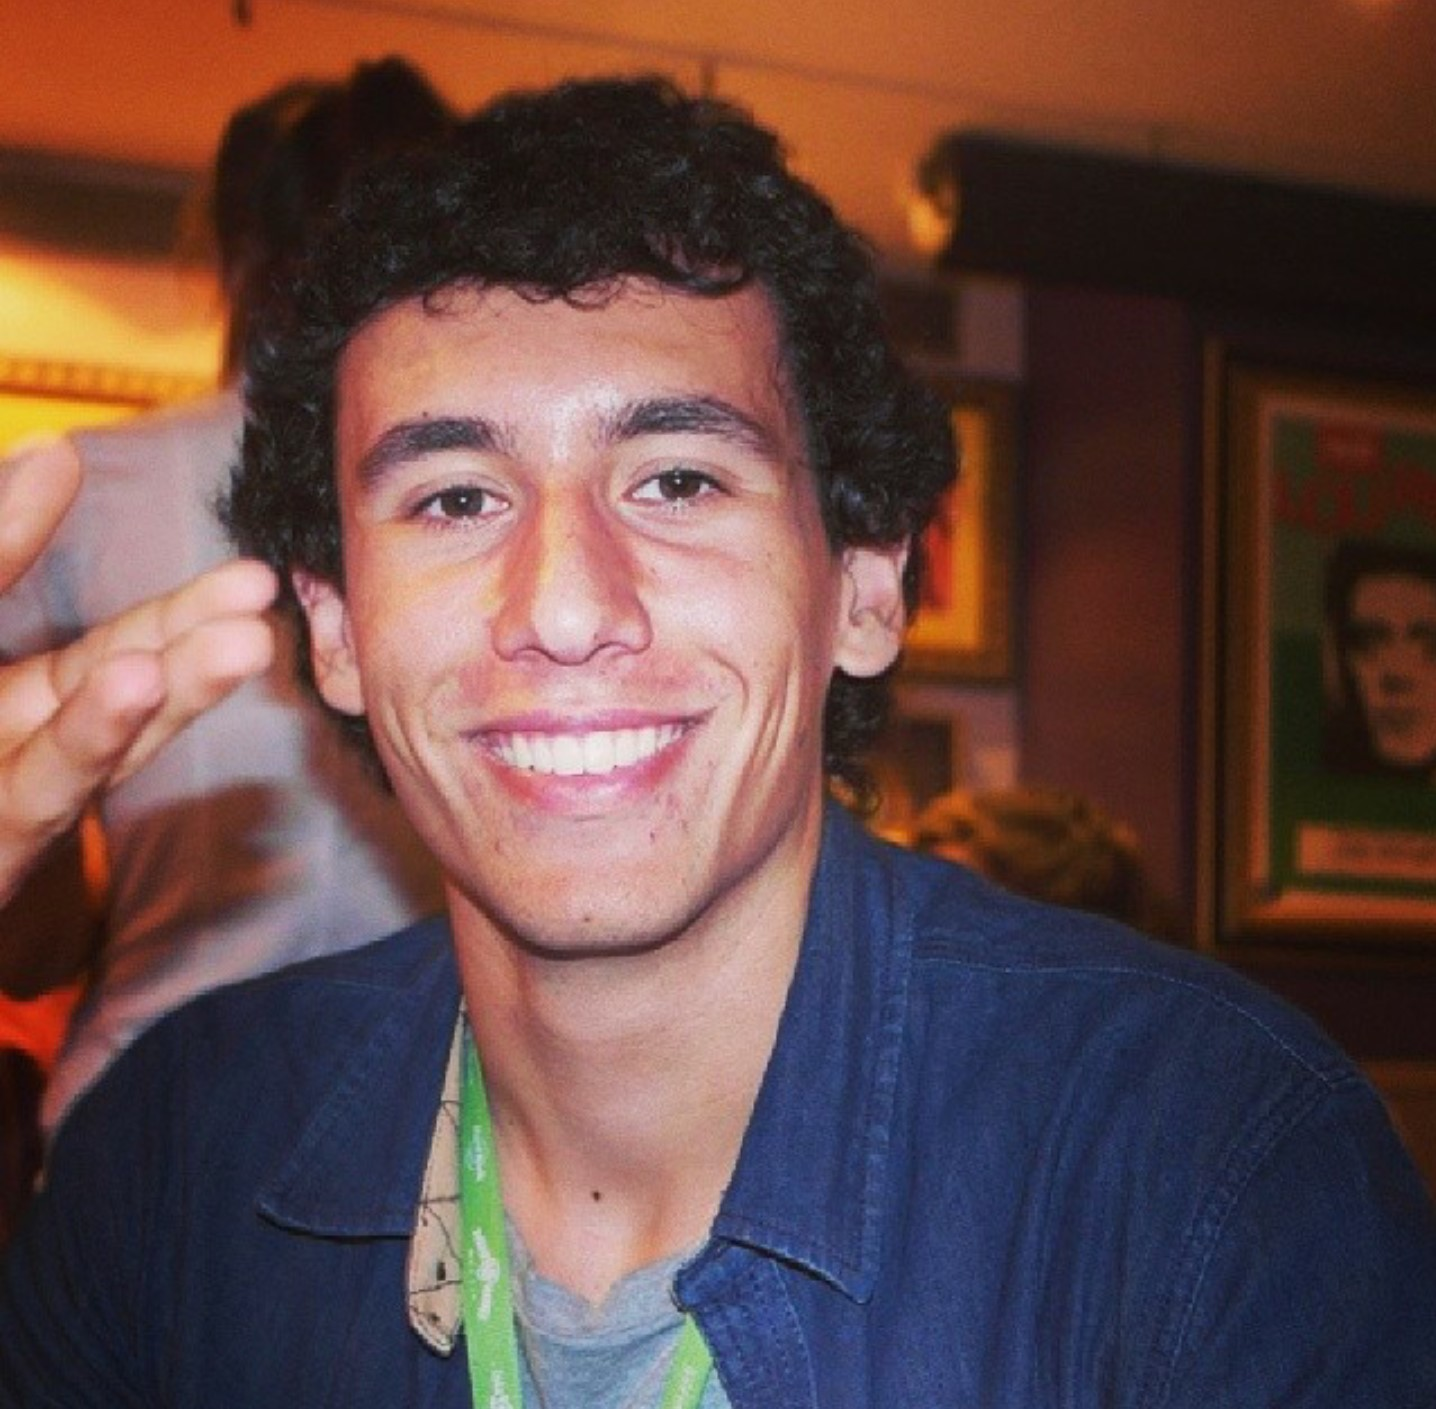
\includegraphics[width=1.5cm]{marco.jpg}\break
  \end{flushleft}
\end{minipage}%
\vfill

% Bottom of the page
{\large Versão 1.0 \\ \today}

\end{center}
\end{titlepage}


\begin{abstract}

\hspace{3mm} 

\end{abstract}

\pagebreak
\tableofcontents

\pagebreak

% ===================================================
\section{Introdução}

\hspace{3mm} 

% ===================================================
\section{Descrição do Trabalho e Análise de Resultados}


% ---------------------------------------------------
\subsection{Generator - Normais} 

\subsubsection{Plano}%[DANIEL]

\hspace{3mm}A geração das normais nos pontos do plano é trivial, graças ao facto de que este é sempre desenhado centrado no plano \textit{xz}. Como tal, foi apenas uma questão de preencher um ponto - sabendo que este será interpretado como um vetor - com a normal (0, 1, 0), visto que o plano é desenhado de modo a ser visível a partir da sua face superior. Seguidamente, guarda-se esta normal para cada ponto do plano.

\subsubsection{Box}%[DANIEL]

\hspace{3mm}A geração dos normais da \textit{box} assemelha-se à do plano, no sentido em que se trata de um conjunto vetores unitários alinhados a um eixo de coordenadas. No caso da \textit{box}, varia também qual dos eixos adquire o valor unitário e o sinal do mesmo. Este depende de qual das faces está a ser desenhada.

Sendo assim, o domínio de possíveis valores das normais dos pontos da \textit{box} são os seguintes:
\begin{itemize}
    \item (0, 0, 1) se se tratar da face paralela ao plano \textit{xy} orientada para o lado positivo do eixo \textit{z};
    \item (0, 0, -1) se se tratar da face paralela ao plano \textit{xy} orientada para o lado negativo do eixo \textit{z};
    \item (0, 1, 0) se se tratar da face paralela ao plano \textit{xz} orientada para o lado positivo do eixo \textit{y};
    \item (0, -1, 0) se se tratar da face paralela ao plano \textit{xz} orientada para o lado negativo do eixo \textit{y};
    \item (1, 0, 0) se se tratar da face paralela ao plano \textit{yz} orientada para o lado positivo do eixo \textit{x};
    \item (-1, 0, 0) se se tratar da face paralela ao plano \textit{yz} orientada para o lado negativo do eixo \textit{x}.
\end{itemize}

\subsubsection{Cone}%[DANIEL]

\hspace{3mm} A geração das normais do cone pode ser separada em duas partes: a base e a face lateral. 

A formulação das normais da base do cone é simples, sendo que este é essencialmente um plano paralelo a \textit{xz} orientado no sentido negativo relativo ao eixo \textit{y}. Como tal, todos os vértices da base terão uma normal de valor (0, -1, 0).

Por sua vez, para o cálculo das normais da face lateral do cone, recorreu-se à definição do vetor normal, que estipula que este se define pelo produto externo de dois vetores auxiliares. Estes, denominados de $v_1$ e $v_2$, serão tangentes ao plano paralelo ao triângulo que será desenhado numa dada iteração. Para adquirir estes vetores, são utilizados a cada iteração os pontos $p_0, p_1$ e $p_2$, vértices do triângulo a ser desenhado. Com estes, %TO BE CONTINUED --->

\subsubsection{Esfera}%[DANIEL]
\subsubsection{Torus} % [MARCO]

\hspace{3mm} Antes de qualquer explicação teórica, observe-se na imagem abaixo uma representação de alguns dos vetores normais a calcular.

\begin{figure}[!h]
    \centering
    \includegraphics[width=0.5\linewidth]{TorusNormalVector.png}
    \caption{Representação gráfica de alguns vetores normais à superficie do \textit{Torus}.}
    \label{fig:ref_normalTorus}
\end{figure}

Como se pode observar, as normais da superficie do \textit{Torus} são bastante distintas ao longo da superficie, pelo que, foi utilizado o produto vetorial para o cálculo das mesmas. Uma vez que, todas a figuras são constituidas por triângulos, será apenas necessário calcular um vetor normal para cada conjunto de 3 pontos.

Deste modo, foi desenvolvido o seguinte código.

\begin{lstlisting}[language=C++, caption=Código responsável pelo cálculo do vetor normal para um triângulo.]
            p_aux[0].setPoint((radius + (radius_torus * cos(i * increment1))) * cos(j * increment), (radius + (radius_torus * cos(i * increment1))) * sin(j * increment), radius_torus * sin(i * increment1));
            p_aux[1].setPoint((radius + (radius_torus * cos(i * increment1))) * cos((j + 1) * increment), (radius + (radius_torus * cos(i * increment1))) * sin((j + 1) * increment), radius_torus * sin(i * increment1));
            p_aux[2].setPoint((radius + (radius_torus * cos((i + 1) * increment1))) * cos(j * increment), (radius + (radius_torus * cos((i + 1) * increment1))) * sin(j * increment), radius_torus * sin((i + 1) * increment1));

            //Calculo do vetor normal
            v1 = difference(p_aux[1], p_aux[0]);
            v2 = difference(p_aux[2], p_aux[0]);
            normal = normalize( cross(v1, v2) );
\end{lstlisting}

Como se pode observar, numa primeira fase, os pontos do primeiro vértice a desenhar são colocados numa estrutura de dados auxiliar por forma a facilitar os cálculos do vetor normal. Assim, de seguida procede-se ao cálculo dos vetores \textit{v1} e \textit{v2} recorrendo aos pontos presentes na estrutura de dados auxiliar. Finalmente, tendo dois vetores com a mesma origem, procede-se finalmente ao do vetor normal para o triângulo. De salientar também que este deve encontrar-se normalizado.


\begin{figure}[!h]
    \centering
    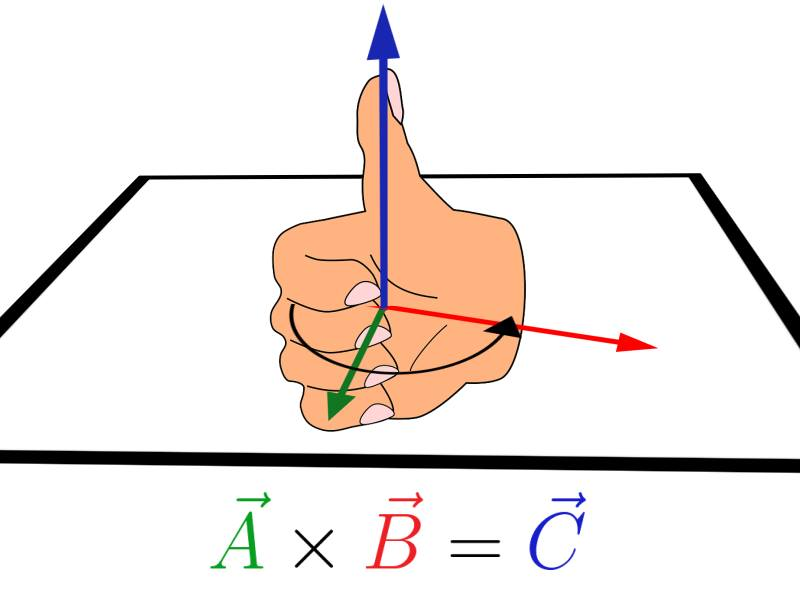
\includegraphics[width=0.5\linewidth]{regra_mao_direita.jpg}
    \caption{Representação gráfica da regra da mão direita utilizada no produto cruzado entre dois vetores.}
    \label{fig:ref_mao_direita}
\end{figure}


\subsubsection{Patch}%[DANIEL]

% ---------------------------------------------------
\subsection{Generator - Coordenadas da textura} 

\subsubsection{Plano}
\subsubsection{Box}
\subsubsection{Cone}
\subsubsection{Esfera}
\subsubsection{Torus}%[MARCO]

\hspace{3mm} Para o revestimento do \textit{Torus}, a textura não foi aplicada diretamente à figura geométrica. Esta abordagem não foi adotada uma vez que iria originar quebras bastante bruscas na cor tornando assim a figura desagradável à vista. Por forma a evitar a situação apresentada anteriormente, decidiu-se dividir a figura horizontalmente ao meio e aplicar a textura completa na parte superior e inferior. Foi também necessário que a aplicação da textura numa das faces fosse feita no sentido inverso por forma a evitar quebras de cor.

Observe-se agora um exemplo de textura para o torus.

\begin{figure}[!h]
    \centering
    
\includegraphics[width=0.5\linewidth]{8k_saturn_ring_alpha.png}
    \caption{Exemplo de textura.}
    \label{fig:ref_texture}
\end{figure}

Para que no \textit{Torus} fosse representado o efeito de inúmeros aneis, optou-se por para cada uma das \textit{slices} proceder-se à aplicação da textura completa. Deste modo, o eixo do \textit{x} da textura ficará representado ao longo das \textit{stacks}. Relativamente ao eixo do \textit{y} da textura, uma vez que em cada uma das \textit{slices} será aplicada uma textura completa, não será necessário efetuar qualquer cálculo para percorrer a textura visto que as coordenadas desta componente apenas tomarão os valores 0 e 1.

Deste modo, na face superior o eixo do \textit{x} da textura será percorrido segundo a seguinte fórmula,

\[ 2 * i * incrementT \]

sendo \textit{i} representativo do número de stacks (na parte superior do \textit{Torus}), \textit{incrementT} o incremento em cada uma das iterações e finalmente

\[ 1 - (2 * texture_aux * incrementT) \]

sendo \textit{texture\_aux} uma variável auxiliar para percorrer a textura do fim para o início.

\begin{figure}[!h]
    \centering
    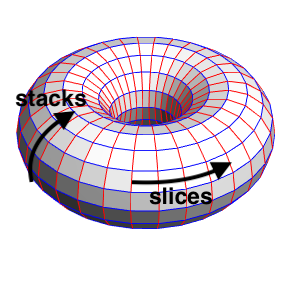
\includegraphics[width=0.5\linewidth]{torus1.png}
    \caption{Ilustração do algoritmo de criação de coordenadas de textura.}
    \label{fig:ref_torus1}
\end{figure}

Deste modo, obtemos o seguinte resultado.

\begin{figure}[!h]
    \centering
    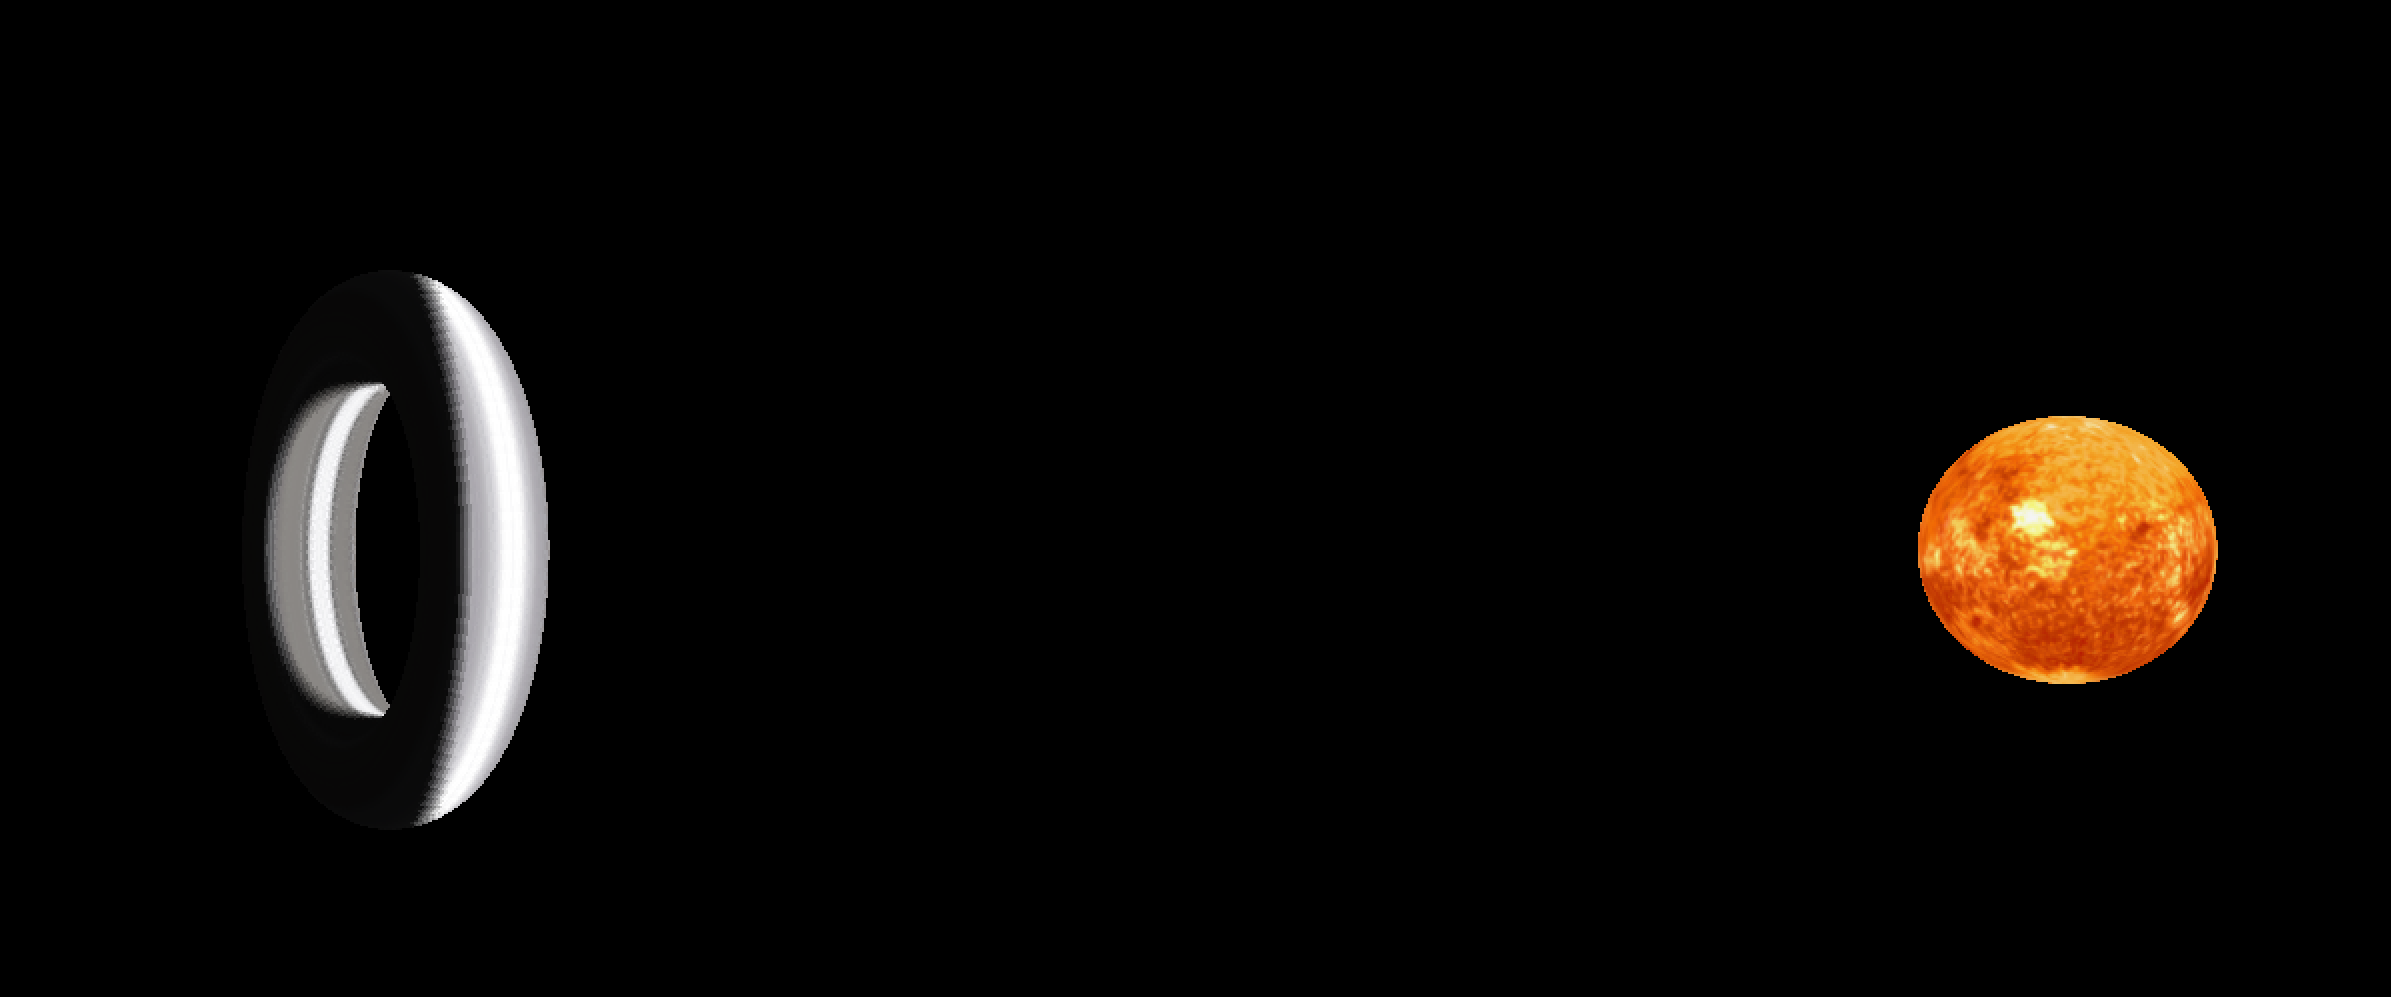
\includegraphics[width=0.5\linewidth]{exemplo_torus.png}
    \caption{Exemplificação da figura \textit{Torus}.}
    \label{fig:ref_ex_torus}
\end{figure}

\subsubsection{Patch}


% ---------------------------------------------------
\subsection{Iluminação} %[AFONSO]

\subsubsection{Directional Light}
\subsubsection{Point Light}
\subsubsection{Spotlight}

% ---------------------------------------------------
\subsection{Fucionalidades Adicionais}

\subsubsection{FPS} %[MARCO]

\hspace{3mm} Tendo em conta a dimensão do modelo do sistema solar desenvolvido, para uma melhor visualização do mesmo, foi implementada a câmara de primeira pessoa, também designada por \textit{FPS (First Person Shooter)}. Este modo de visualização permite ao utilizador explorar livremente o modelo do sistema solar, possibilitando o posicionamento da câmara em qualquer um dos pontos do modelo.

A implementação deste modo de visualização tem como base a utilização de coordenadas esféricas. Deste modo, praticamente toda a computação necessária à implementação desta funcionalidade incidirá sobre o calculo da direção da câmara, ou seja, a direção para onde o utilizador pretende que a câmara se encontre virada. Para que este cálculo seja possível, será necessário manter 3 parâmetros, a posição da câmara em cada um dos instantes, um ângulo $\alpha$ representativo da rotação horizontal da câmara e finalmente um ângulo $\beta$ que caracteriza a elevação vertical do olhar.

\begin{figure}[!h]
    \centering
    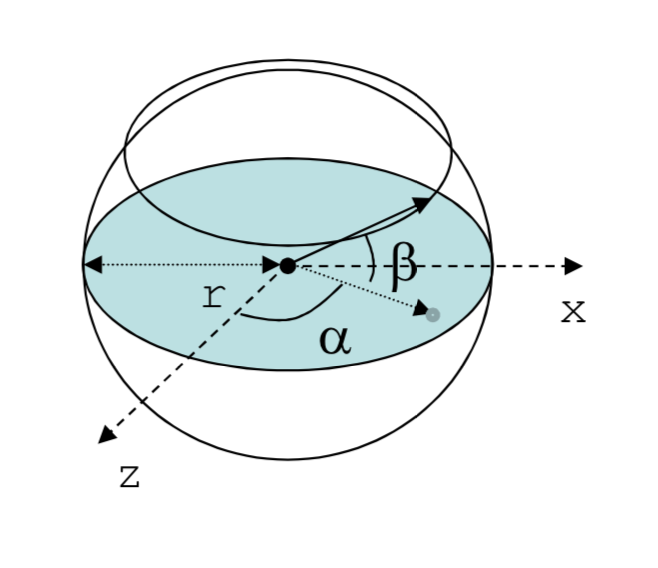
\includegraphics[width=0.5\linewidth]{referencial_FPS.png}
    \caption{Esquema de representação das 3 componentes essencias à implementação da câmara \textit{FPS}.}
    \label{fig:ref_FPS}
\end{figure}

Tendo então bem definidas as 3 componentes, procedeu-se ao cálculo da direção do olhar da câmara. Esta direção será representada por um vetor \textit{D} ficando assim representadas neste vetor as orientações vertical e horizontal, uma vez que, este será computado com base nos ângulos anteriormente mencionados $\alpha$ e $\beta$.

Por forma a obter resultados mais precisos e com o menor esforço computacional possível, este vetor \textit{D} deverá encontrar-se sempre normalizado. Consequentemente, considere-se este último de comprimento 1 e sempre com origem na posição atual da câmara. Vejamos então a imagem abaixo para uma melhor compreensão do cálculo a executar.

\begin{figure}[!h]
    \centering
    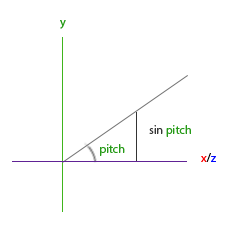
\includegraphics[width=0.5\linewidth]{camera_pitch.png}
    \caption{Representação do vetor de direção do olhar da câmara, sendo o ângulo \textit{pitch} representativo de $\beta$.}
    \label{fig:ref_FPS1}
\end{figure}

Como resultado da observação das imagens apresentadas acima, percebeu-se facilmente que o vetor \textit{D} pode ser calculado da seguinte forma.

\[ dx = sin(\alpha) \]
\[ dy = sin(\beta) \]
\[ dz = cos(\alpha) \]

Tendo calculado o vetor direção do olhar, este terá de ser aplicado na função \textit{gluLookAt}, de modo a que a direção do olhar seja aplicada à câmara. Deste modo, iremos ter a função \textit{gluLookAt} com o seguinte formato.

\begin{lstlisting}[language=C++, caption=Definição da função \textit{gluLookAt}.]
        gluLookAt(px, py, pz,
                  px + dx, py + dy, pz + dz,
                  ux, uy, uz);
\end{lstlisting}

Como se pode ver acima, encontram-se definidas 3 componentes distintas. Nos primeiros 3 campos, são definidos os valores para as componentes de posição da câmara, seguidos do vetor direção e finalmente o vetor \textit{up}. Pode-se ver agora o vetor direção definido como a soma da posição atual da câmara com o vetor anteriormente computado com base nos ângulos $\alpha$ e $\beta$ como já tinha sido referido anteriormente. Note-se também que neste caso, não é necessário efetuar qualquer cálculo para as componentes do vetor \textit{u}, tomando as suas componentes \textit{x}, \textit{y} e \textit{z} os valores 0, 1 e 0 respetivamente.

Por forma a permitir o deslocamento da câmara, foram definidas duas funções responsáveis pela atualização da posição da câmara com base no vetor direção, como podemos ver abaixo.

\begin{lstlisting}[language=C++, caption=Definição das funções responsáveis pelo movimento para frente e trás da câmara.]
        void moveforward(){

            px = px + 0.5 * dx;
            py = py + 0.5 * dy;
            pz = pz + 0.5 * dz;

        }

        void movebackwards(){

            px = px - 0.5 * dx;
            py = py - 0.5 * dy;
            pz = pz - 0.5 * dz;

        }
\end{lstlisting}

\begin{figure}[!h]
    \centering
    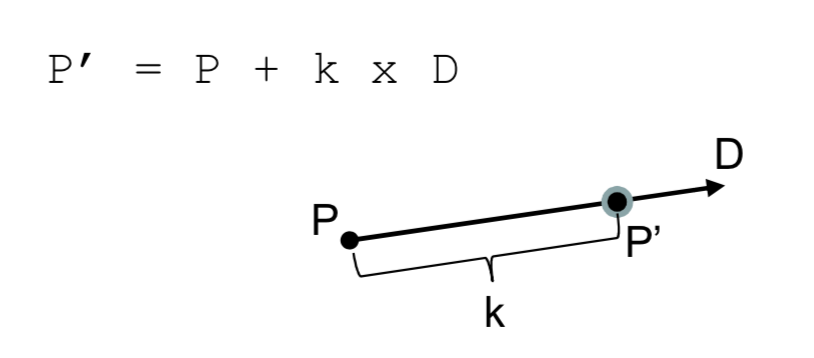
\includegraphics[width=0.5\linewidth]{referencial_FPS2.png}
    \caption{Esquema representativo do movimento da câmara.}
    \label{fig:ref_FPS3}
\end{figure}

Finalmente, foram definidas teclas que permissem a alteração de todos os parâmetros referidos anteriormente. Vejamos então as funções \textit{movement} e \textit{keyboard}.

\begin{lstlisting}[language=C++, caption=Definição das funções responsáveis pelo movimento para frente e trás da câmara.]
        void keyboard(unsigned char key, int x, int y){

            (...)

            if (key == 'n')
                move = (move + 1) % 2;

            if (key == ' ')
                moveforward();

            if (key == 'b')
                movebackwards();

            (...)
        }

        void movement (int key, int x, int y) {

            switch (key) {
                case GLUT_KEY_LEFT :
                    alfa += 0.1f;
                    break;
                case GLUT_KEY_RIGHT :
                    alfa -= 0.1f;
                    break;
                case GLUT_KEY_UP :
                    beta1 -= 0.08f;
                    if (beta1 < M_PI / 2)
                        beta1 = M_PI / 2;
                    break;
                case GLUT_KEY_DOWN :
                    beta1 += 0.08f;
                    if (beta1 > 3 * M_PI / 2)
                        beta1 = 3 * M_PI / 2;
                    break;
            }
        }
\end{lstlisting}

Como se pode observar, as setas serão utilizadas para o movimento da câmara fazendo variar os ângulos $\alpha$ e $\beta$. Para além destas, foi definido também o espaço para o movimento unitário para a frente. De uma forma semelhante, a tecla \textit{b} foi mapeada para o movimento contrário. Finalmente, para comodidade do utilizador, a tecla \textit{n} encontra-se mapeada com uma opção de movimento em frente automático, possíbilitando assim ao utilizador alterar a direção de movimento enquanto se desloca para em frente. Esta ação não é possível com a tecla \textit{espaço} devido à impossibilidade de deteção de duas teclas premidas ao mesmo tempo por parte do \textit{OpenGL}.

Numa fase final do projeto, foi também implementada a funcionalidade de alteração da direção do olhar da câmara com o rato para uma interação do utilizador com o \textit{engine} ainda mais natural. Para a implementação desta funcionalidade, recorreu-se ao código fornecido pelos docentes nas aulas práticas utilizado na implementação da câmara de explorador que utilizava o rato como modo de interação com o utilizador.

Uma vez que este código já calcula o deslocamento do rato quando premido, apenas foi necessário com alguns testes encontrar um fator que tornasse a experiência agradável para o utilizador e adicionar esse deslocamento multiplicado pelo fator anteriormente referido às variáveis já definidas $\alpha$ e $\beta$. Deste modo, apenas se acrescentaram as seguintes linhas de código à função \textit{processMouseMotion}.

\begin{lstlisting}[language=C++, caption=Alterações na função \textit{processMouseMotion}.]
 
         (...)

         if (tracking == 1) {
                alfa += 0.001 * -(xx - startX);
                beta1 += 0.001 * (yy - startY);

                alphaAux = alpha + deltaX;
                betaAux = beta + deltaY;

         (...)

\end{lstlisting}



%Não sei se temos mais alguma
%temos a parte das teclas a ligar e desligar
%temos o fundo com as estrelas
%ativação das orbitas

% ---------------------------------------------------
\subsection{Resultado Final} %[AFONSO]



\clearpage
% ===================================================
\section{Conclusões e Sugestões} 

\hspace{3mm} 


\newpage
% =========================================================
\bibliographystyle{unsrt}
\bibliography{biblio}

\newpage
% ===================================================
\section{Anexos}

\begin{lstlisting}[language=XML, caption=Ficheiro \emph{XML} de modelação do sistema solar.]
    
\end{lstlisting}



\end{document}
